\section{Pregunta N$^{\circ}$7\qquad Leon Alonzo Terrones Caccha}

\begin{frame}
    \begin{enumerate}\setcounter{enumi}{6}
        \item

              Use
              \begin{math}
                  f\left(x\right)=
                  \cos\left(3x^{2}\right)-
                  x^{2}
              \end{math}
              para obtener la aproximación de mínimos cuadrados
              discretos $S_{2}\left(x\right)$ para los datos
              \begin{math}
                  \left\{
                  \left(x_{j},y_{j}\right)
                  \right\}_{j=0}^{11}
              \end{math},
              donde $x_{j}=\dfrac{2\pi j}{m}-\pi$ y
              $y_{j}=f\left(x_{j}\right)$ en el intervalo
              $\left[-\pi,\pi\right]$.
    \end{enumerate}

    \begin{solution}
        Deseamos obtener un polinomio trigonométrico de la forma:
        \[S_{2}\left(x\right)=\frac{a_{0}}{2}+a_{2}cos(2x)+a_1cos(x)+b_1sen(x)\]
        donde:
        \[a_k=\frac{1}{6}\sum_{j=1}^{11}{y_jcos(kx_j)}\]
        \[b_k=\frac{1}{6}\sum_{j=1}^{11}{y_jsen(kx_j)}\]
    \end{solution}
\end{frame}
\begin{frame}{Results}
    \begin{figure}
        \centering
        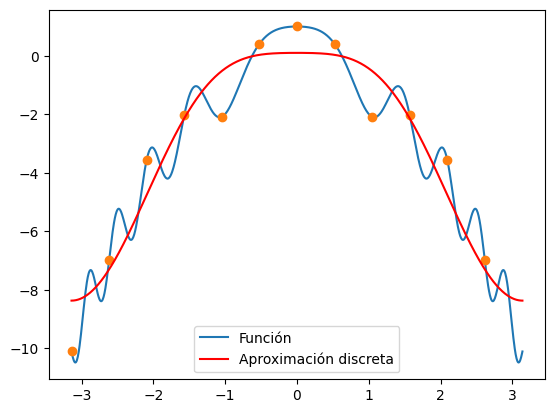
\includegraphics[width=8]{p7-Aprox-discreta.png}
        \caption{Para $n=2$ y $m=6$}
        \label{fig:enter-label}
    \end{figure}
\end{frame}
\begin{frame}{Results}
    \begin{figure}
        \centering
        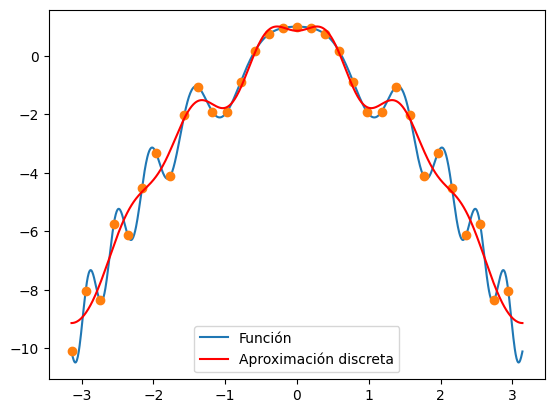
\includegraphics[width=8]{p7-A-discreta2.png}
        \caption{Para $n=7$ y $m=16$}
        \label{fig:enter-label}
    \end{figure}
\end{frame}
\begin{frame}{Results}
    \begin{figure}
        \centering
        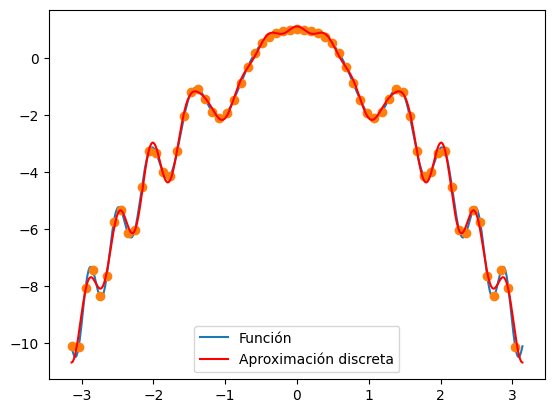
\includegraphics[width=8]{p7-A-discreta3.png}
        \caption{Para $n=15$ y $m=32$}
        \label{fig:enter-label}
    \end{figure}
\end{frame}